\section{Vectorización}
La red hasta este momento solo había sido representada mediante nodos, ahora vamos a hacer el uso de una notación en particular la cúal consta de matrices y vectores. Para generalizar nuestras fórmulas en la derivación matemática. %, del grediente se hizo considerando que tuviéramos un solo ejemplar de entrenamiento pero realmente vamos a entrenar a nuestra red con varios ejemplares. 

Consideremos todos los datos involucrados durante el entrenamiento:
\begin{enumerate}
 \item Hay $S_{L}$ neuronas de salida, para las cuales se calculará el error.
 \item Se puede calcular el promedio del gradiente para m ejemplares simultáneamente.
 \item Si escribimos los datos en forma matricial, es posible paralelizar estos cálculos utilizando operaciones de matrices.
\end{enumerate}
Denotemos nuevamente nuestra función de error:
 \begin{equation}
  J (\Theta) = -\dfrac{1}{m}\left[\sum_{i=1}^{m}\sum_{k=1}^{s_{L}}y_{k}^{i} log( h_{\Theta}(x^i))_{k}+(1-y_{k}^{i})log(1- h_{\Theta}(x^i))_{k}  \right]  
 \end{equation}

Ahora con nuestros datos en forma matricial:
\begin{equation}
X = 
\begin{pmatrix}
x_{0}^{(1)} & \cdots & x_{n}^{(1)}\\
\vdots & \ddots & \vdots\\
x_{0}^{(m)} & \cdots & x_{n}^{(m)}\\
\end{pmatrix}
\end{equation}


\begin{equation}
Y = 
\begin{pmatrix}
y_{0}^{(1)} & \cdots & y_{S_{L}}^{(1)}\\
\vdots & \ddots & \vdots\\
y_{0}^{(m)} & \cdots & y_{S_{L}}^{(m)}\\
\end{pmatrix}
\end{equation}


\begin{equation}
\Theta^{(l)} = 
\begin{pmatrix}
\Theta_{01} & \cdots & \Theta_{0s_{l}}\\
\vdots & \ddots & \vdots\\
\Theta_{(s_{(l-1)}1)} & \cdots & \Theta_{(s_{(l-1)}Sl)}\\
\end{pmatrix}
\end{equation}

Podemos reescribir:
\begin{equation}
 \delta_{k}^{(L)}=(y_{k}-a_{k}^{(L)})
\end{equation}

\begin{align*}
\delta_{k}^{(L)}&=(y_{k}-a_{k}^{(L)})           &  \Delta^{(L)}&=Y-A^{(L)}
\end{align*}

\begin{align*}
 \dfrac{\partial J}{\partial\theta_{jk}^{L-1}}&=-\dfrac{1}{m}\sum_{i=1}^{m}a_{j}^{(L-1)(i)}\delta_{k}^{(L)(i)}             &  \nabla^{(L-1)}&=-\dfrac{1}{m}\left(A^{(L-1)}\right)^{T} \Delta^{L}
\end{align*}

\begin{align*}
\delta_{j}^{(L-1)}&=\left(\sum_{k=1}^{s_{L}} \delta_{k}^{(L)}\theta_{jk}\right)g'(z_{j})           &  \Delta^{(L-1)}&=\Delta^{(L)}\left(\Theta_{[1:,:]}^{(L-1)}\right)^{T} \circ g'(Z^{(L-1)})
\end{align*}

\begin{align*}
 \dfrac{\partial J}{\partial\theta_{jk}^{L-2}}&=-a_{i}^{(L-2)}\delta_{j}^{(L-i)}             &  \nabla^{(L-2)}&=-\dfrac{1}{m}\left(A^{(L-2)}\right)^{T} \Delta^{L-1}
\end{align*}

Vectorización 3

Las fórmulas vectorizadas se pueden escribir en forma general con: \emph{Error cometido por la última capa L.}
\begin{equation}
 \Delta^{(L)} = Y-A^{(L)}
\end{equation}

\emph{Error cometido por cualquier capa l − 1.}
\begin{equation}
  \Delta^{(L-1)}=\Delta^{(L)}\left(\Theta_{[1:,:]}^{(L-1)}\right)^{T} \circ g'(Z^{(L-1)})
\end{equation}

\begin{equation}
 g' (Z^{(l-1)}) = A^(l-1) \circ (1-A^{(l-1)})
\end{equation}

Componentes del gradiente con respecto a los pesos en $\Theta^{l-1}$.
\begin{equation}
  \nabla^{(L-1)}=-\dfrac{1}{m}\left(A^{(L-1)}\right)^{T} \Delta^{L}
\end{equation}

Nuestra formula de error, es un promedio de la suma de errores que se tuvo en cada ejemplar $(i)$ del total de ejemplares $m$.
Para poder empezar a trabajar con matrices vamos a empezar a ver cómo están escritos nuestros datos todo recordemos como habíamos dicho que íbamos a escribir nuestras entradas de entrenamiento la idea es que cada ejemplar es un renglón tenemos n características, está pensando en que estamos agregando aquí los sesgos y después  lo que ocurre con nuestras etiquetas de clasificación recordemos que en redes neuronales utilizamos el one hot en coding. Entonces aunque si tenemos cinco clases tenemos cinco neuronas de salida y eso quiere decir que nuestra etiqueta tiene algo así este sería una etiqueta en la que la clase correcta es la que está en la tercera neurona otro ejemplar podría ser de esta manera y pues aunque solamente haya uno que sea distinto de cero la forma en la que van a venir empaquetadas nuestras respuestas correctas va a ser precisamente en forma de matriz donde tenemos sobre los renglones tantos bits como neuronas haya en la última capa y tenemos hacia abajo los m ejemplares de entrenamiento después recordemos cómo teníamos escritas las matrices de pesos teníamos por cada columna los pesos que contribuyen a la a una neurona en la siguiente capa entonces sobre cada renglón tendríamos a tener tantos pesos como neuronas haya en la capa cl y hacia abajo vamos a tener tantos pesos como neuronas había en la capa $sl -1$ y que contribuyeron al siguiente elemento en ese l .
Así que tendríamos a las diferentes neuronas que van a estar en nuestra nueva capa eso es lo que va a hacer es que cuando multipliquemos x y z nos queden otra vez los valores de cada en la siguiente capa con los renglones correspondientes a los ejemplares de entrenamiento y horizontalmente los valores de activación de cada neurona en la siguiente bien entonces partes importantes ejemplares de entrenamiento hacia abajo para estos dos aquí el décima capa hacia acá está para l menos uno ahora están copiadas acá del lado izquierdo las fórmulas tal y como las obtuvimos ejemplar por ejemplar y lo que vamos a hacer ahora es escribirlas en forma matricial bueno que ya me adelanté ya se las escribí entonces va a ser más fácil. Lo que estamos viendo aquí para eso voy a utilizar ahora otro programa y aquí está vamos a utilizar aquí para que pueda dibujar qué es lo que está primero que teníamos en delta está en la capa no en la capa l bueno voy a dibujar aquí ahorita una pequeña red neuronal en este conector y entonces nos estamos preguntando por qué pasa con él aquí está él bueno lo que decíamos era que vamos a tener una de estas del estás por cada uno de nuestras neuronas de salida y lo que vamos a ver es qué tenemos los ejemplares hacia abajo y las neuronas horizontales los valores que tengo aquí verticalmente los acosté y es lo que tengo acá ya vimos también entonces que la llega realmente tiene varios bits horizontalmente y la sas también entonces si yo restó enrique menos acá observen que esto en realidad es un vector tengo una componente por cada neurona de salida entonces aunque aquí les saquemos componente por componente pues tengo uno de cada uno. 
El hacer las combinaciones de todos contra todos es cuando obtengo el efecto que ocurrió con cada peso pero quiero sumar estos productos para todos los ejemplares de entrenamiento y sumarlos bueno eso es prácticamente lo que hace una multiplicación de matrices ahora para poder hacer todo esto en un solo paso lo que tenemos que hacer es acomodar las acorde mente nos vamos a hacer lo siguiente ya habíamos dicho que esta delta que realmente tiene forma de matriz como ésta de tal manera que mira aquí hacia acá tenemos todos los es el es y así aquí abajo tenemos todos nuestros ejemplares de entrenamiento bueno y que sabemos de la aj y también son los valores de activación y queremos combinar cada j de cada ejemplar de entrenamiento con su respectiva que del mismo ejemplar de entrenamiento y después multiplicarlos y sumarlos bien entonces vamos a acomodar a la sas de la siguiente manera y vamos a poner hacia acá a los ejemplares de entrenamiento y así acá a los elementos son ordenadas iba a suceder si yo hago esto observen que se multiplican ejemplares de entrenamiento contra ejemplares de entrenamiento misma aj contra mismos del tak as pero de diferentes ejemplares de entrenamiento cada uno con su respectivo y además se suman para definir la coordenada que va a quedar aquí cuando yo tomé este contra la siguiente columna entonces otra vez vamos a estar multiplicando en ejemplares contra mi ejemplares los vamos a sumar y nos va a dar el dato que tengamos aquí los conservamos las columnas que teníamos acá s l cuando empiece a hacerlo con los renglones voy a tener entonces lo que ocurre con las s menos el c lm no son tan clones que teníamos acá y esto es sumamente interesante porque esto que está aquí debería de resultarnos un poco conocido sl sl - solo vamos a ver que teníamos acá sl sl - 1 tiene exactamente la misma forma en la matriz de pesos y no es coincidencia recordemos que es lo que estamos tratando de calcular estamos tratando de calcular el gradiente el ingrediente es la parcial con respecto a cada uno de los pesos entonces lo que acabamos de obtener es ese gradiente que tiene acomodadas cada una de las parciales en la posición que corresponde al mismo peso pero en la matriz de pesos bastante bonito muy bien entonces por eso cuando ponemos la matriz a él pero transpuesta para que tengamos ahora si los ejemplares de entrenamiento de forma horizontal. 

Entonces podemos obtener en una multiplicación de matriz todos los componentes del gradiente para los pesos en esa capa lo que ocurre con las siguientes bueno de hecho con los siguientes gradientes es que se van a hacer exactamente igual lo único que nos queda ligeramente entretenido es cómo vamos a calcular los errores de las capas intermedias hay entonces que observar lo siguiente en primer lugar las ventas van a tener la misma forma que éste es que primas entonces simple y sencillamente van a ser dos matrices donde se tienen que multiplicar componentes a componentes las vamos a poner con este símbolo que significa circo digo se llama cirque y significa multiplicación componente a componente entre estas dos matrices ahora como vamos a escribir ésta se parece a lo anterior pero ahora sobre lo que queremos es sumar es sobre las neuronas de salida recordemos que la contribución al error de una neurona de la capa intermedia pues es la suma sobre los errores a los que contribuyó en todas las neuronas en la capa siguiente entonces del ejercicio anterior ya debemos de ver como pista en que si queremos hacer una suma sobre estos elementos pues como que esto es lo que vamos a tener que tener en la parte horizontal de la primera matriz y vertical de la segunda entonces de aquí empiezan a salir precisamente los tips de cómo escribir estas 2 estás deltas pues ya tienen automáticamente de manera horizontal lo que está ocurriendo con cada una de las neuronas entonces se quedan exactamente iguales y lo que estaba ocurriendo con los pesos es que entonces vamos a crear los componentes de ese l sobre los renglones los necesitamos tomar la transpuesta para que cumpla con esa condición y en principio y básicamente ya quedaría que ese entonces está en notación extraña que tenemos en la parte de abajo recordemos que si estamos utilizando sesgos si estamos utilizando sesgos tenemos una neurona en esta capa que no está conectada en nadie con nadie en la parte de atrás entonces no existen pesos que hayan hecho que las neuronas de acá contribuyan al error de esta ésta no tenía error es un sesgo entonces aquí no hay nada que calcular por eso lo que tenemos que hacer en la parte de aquí es quitar a los elementos que corresponderían a las así pues el hecho de que los riesgos no están conectados con la capa anterior es básicamente lo que nos está diciendo es que quitemos de la matriz de pesos a todas las conexiones que parten de esta neurona porque estas conexiones pues no bueno ésta no va a estar contribuyendo cada día más bien las que estén en esta capa no están contribuyendo al error de esta neurona entonces lo que ocurra con esta neurona. 
Finalmente para los componentes del gradiente  lo único que vamos a hacer era multiplicar los valores de activación de la capa anterior por los errores de la capa siguiente y eso nos iba a dar ahora sí la participación del gradiente para cada uno de los pesos y esto lo podemos repetir obteniendo uno de una matriz de estos por cada matriz de pesos que hayamos utilizado los con esta técnica básicamente obtenemos el gradiente de pequeños bloques hitos de material de matrices una matriz por cada matriz de pesos si quieren escribir el gradiente entonces como se escribe usualmente en cálculo es como un solo vector pues lo que hay que hacer es aplanar todas esas pequeñas matrices y poner cada una de las componentes en una componente del vector y nos va a quedar un vector gigantesco que tiene tantas tantas componentes como la suma de componentes en todas estas matrices bien y con eso quedaría todo. 
Lo que  se acaba de calcular es el gradiente y cuando nosotros hallamos descenso por el gradiente, lo que necesitamos es la dirección inversa, por eso el signo negativo. Entonces finalmente podemos decir en lo qué consiste el algoritmo de propagación hacia atrás, lo único que estamos haciendo es obtener los ejemplares de entrenamiento las respuestas correctas necesitamos saber cuántas que pasan vamos a inicializar nuestras matrices de errores con ceros bueno podremos hacer lo mismo también con las del gradiente empezamos en la haciendo feedforward que es lo que nos indican estas primeras líneas asignando nuestros datos de entrenamiento a la primera capa la capa de chocolate a partir de ahí utilizamos feedforward para ir calculando todos los valores de activación de las siguientes capas hasta llegar a la última y a partir de ese momento podemos empezar a trabajar ahora sí con el entrenamiento de la red. Tomar en cuenta que era lo que queríamos para sustituir en los cálculos de los errores y los gradientes con las fórmulas que tenemos en la parte de atrás y nos importó precisamente las etiquetas y ya que tenemos. Entonces podemos actualizar, ahora si nuestros pesos en paralelo tienen que actualizarse todos al mismo tiempo no para actualizar primero unos y después otros porque eso ya no es el gradiente en paralelo, tenemos que actualizar tomando los pesos que ya teníamos menos alfa por el gradiente de la función de error, repitiendo esto el suficiente número de veces. La idea es que eventualmente estos pesos nos permitan encontrar un mínimo de la función de error.

Así el algoritmo queda de la siguiente forma:
\begin{figure}[H]
 \centering
 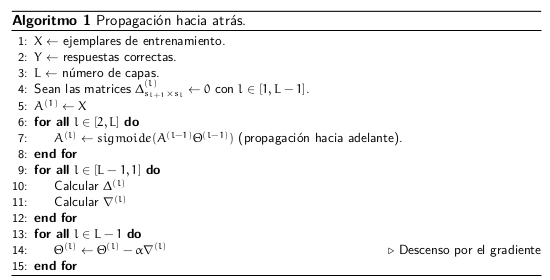
\includegraphics[scale=0.8]{../Figuras/Algoritmo1.png}
 \caption{Algoritmo de retropropagación.}
 \label{fig:algoritmo}
\end{figure}

